\chapter{Introduction}

\section{Context}

Artificial intelligence (\acrshort{ai}) and, more specifically, \acrfirstit{ml} has been through quite a journey since its inception in the 1940s and 1950s. From a small research domain, it has grown into a massive rapidly-developing field of research and applications with ramifications in many branches of science and technology. This growth is not surprising in a world where computers become more and more powerful and data, the bread-and-butter of machine learning, is becoming increasingly collectable, structured, available and queryable. Applications of \acrlong{ml} are as varied as they are numerous: spam filtering, fraud detection, face recognition, self-driving cars, robotics and automation, medical data analysis and diagnosis, simulation in particle physics... to name only a few. While it has already revolutionized many domains, \acrlong{ml} research has still a bright future ahead. In the last decade only, along with \acrfirstit{dl}, several new family of techniques have been (re-)discovered and have enabled unexpectedly-fast progress (\eg \acrlong{cnn}, \acrlong{gan}, transformers). One can only expect that the next ground-breaking \acrshort{ml} method is on the brink of being discovered in a research lab somewhere around the world. Aside from that, research is still ongoing of many fronts such as understanding, applying or improving existing methods.

Medicine is among the numerous fields where \acrlong{ml} is showing great promises. Although often misrepresented in the mainstream media as a tool that will eventually replace practitioners, the real potential of \acrlong{ml} in medicine actually lies in its capacity to become a strong, resilient and consistent assistant to the physicians \parencite{rajkomar2019machine}, assisting them for tasks ranging from diagnosis and analysis to paperwork. Rather than replacing physicians, an \acrshort{ai}-based diagnosis system would be able to complement their opinion and advise them based on experiences of millions of other patients and colleagues. Moreover, such a system would be able to produce these advice based on a very large number of parameters and sources of data that a human could not realistically consider (imaging, written reports, laboratory values, vital signs). However, the road to an \acrshort{ai}-assistant is still long and many questions and challenges have yet to be addressed. From a scientific standpoint, current research mostly focuses on improving solutions for tasks of significantly smaller scale and scope (\eg outlining organs in x-rays, detecting disease in \acrshort{ct}-scans, classifying skin cancer as malignant or benign \TODO{non imaging example}). Many recent contributions, although some arguably lacking scientific rigor, have claimed to have matched or surpassed human experts accuracies by applying machine and \acrlong{dl} methods on different medical tasks \parencite{nagendran2020artificial}. Whereas progress is certain, many challenges have yet to be solved. 

One of these major challenges is \textit{data scarcity}. Not that data itself is lacking as \parencite{pramanik2019healthcare} reported that the amount of health data stored worldwide could reach 2,258 exabytes in 2020. What is scarce is actually data that is at least partially annotated and of good-enough quality to be used to train \acrlong{ml} models. Data scarcity has many causes: privacy concerns prevent sharing patient data, the annotation process is time-consuming and expensive... The usage of \acrlong{dl} makes it even worse as \acrshort{dl} methods are very data-hungry.

In this thesis, we are interested in one specific field of medicine and, more specifically, medical imaging: \acrfirstit{dp}. Microscope have been used in medicine to analyse samples (\eg cells, tissue or blood) since the 17th century \parencite{hajdu2002first} but recent technological progress has enabled the digitization of microscope glass slides into images called \textbf{\acrlong{wsi}s} (\acrshort{wsi}). Digital pathology concerns all the aspects of acquiring, managing, sharing and interpreting these \acrshort{wsi}s \parencite{doolan2019whatisdp}. With the help of image management systems and new visualization tools, \acrshort{wsi}s have greatly facilitated the day-to-day work of practitioners (\eg pathologists, biologists) who do not have to manipulate physical glass slides anymore. More importantly, the digitization has opened the way for \textit{automated analysis} with computer vision techniques, including \acrlong{ml} \parencite{ciompi2021editorial}. Whereas acquiring and managing \acrshort{wsi}s provide interesting challenges, our contributions focus mostly on (automated) analysis and, throughout the thesis, we will refer to this part when using the term \quoteit{\acrlong{dp}}.

\begin{figure}
  \centering
  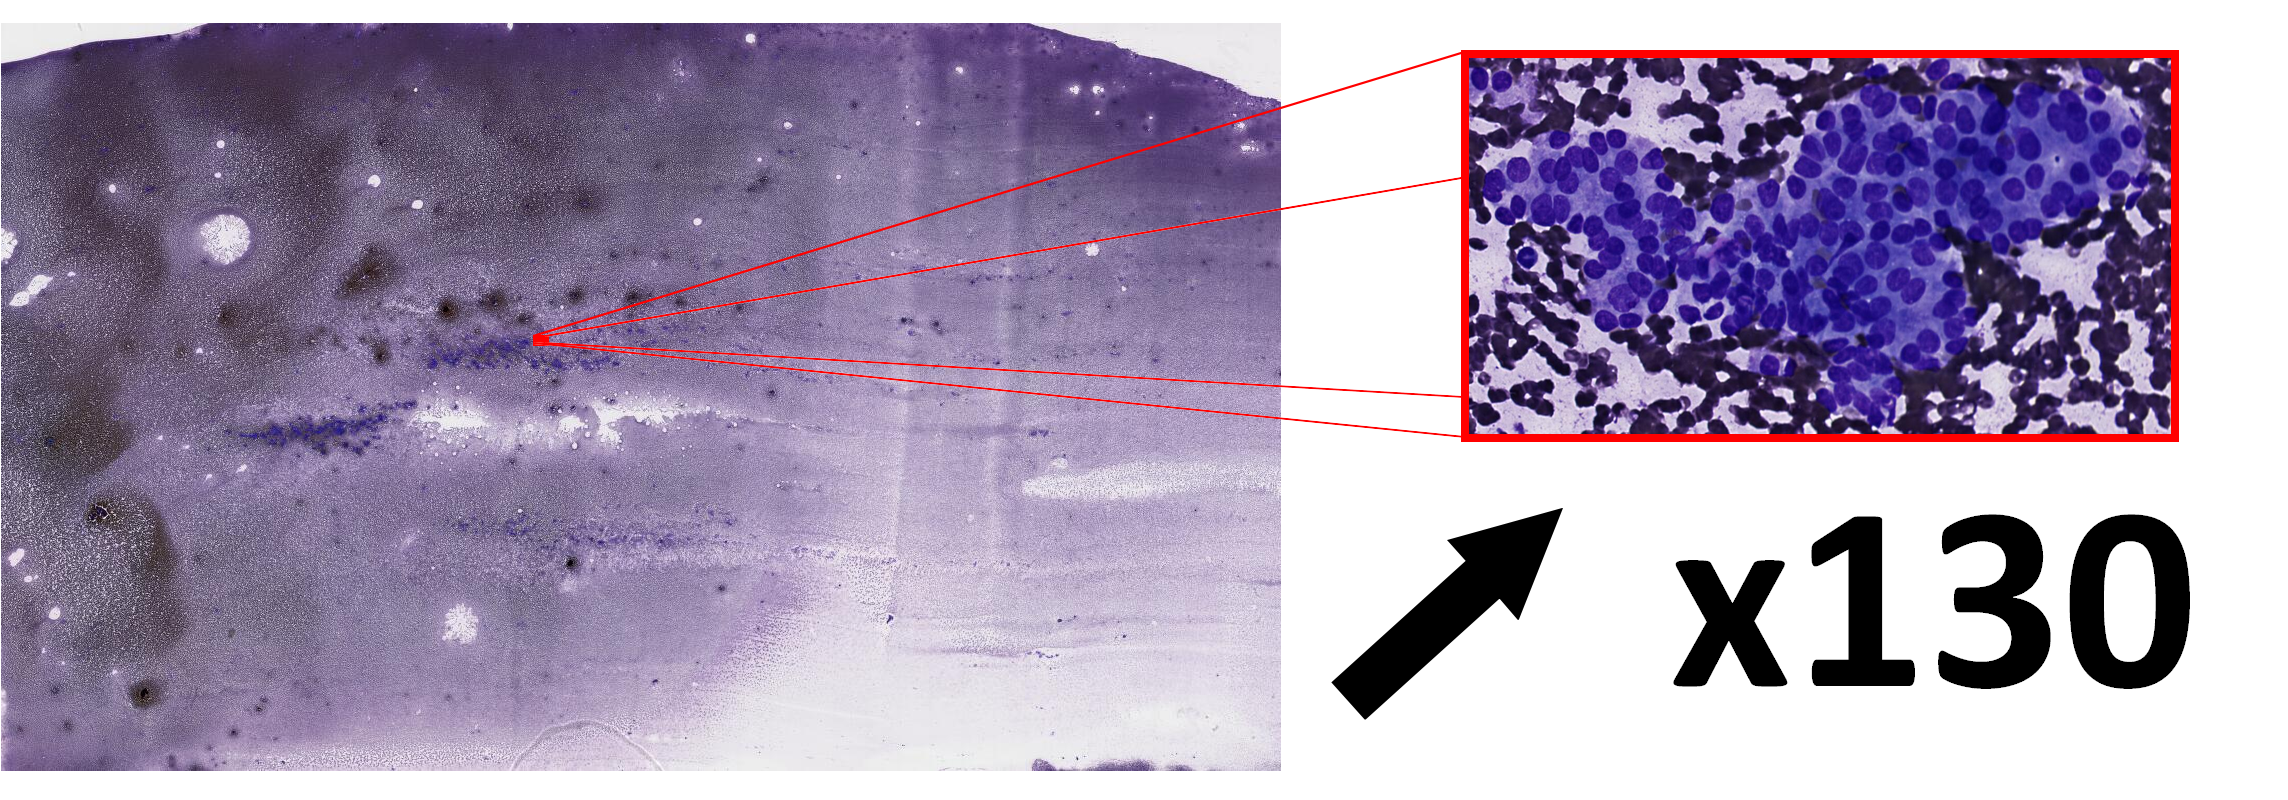
\includegraphics[scale=0.25]{intro/whole-slide-dim.png}
  \caption{A typical \acrlong{wsi} of size 163840 $\times$ 95744 pixels and file size of 2.3 gigabytes. To the left is the original slide and to the right is a structure of interest at zoom level $\times130$ (size in pixels: 1354 $\times$ 736)}.
  \label{fig:intro:wsi}
\end{figure}

Automating the analysis of \acrshort{wsi}s is quite a challenge. Typically, a \acrshort{wsi} is a very large image that can reach few billion pixels at minimum zoom level (see Figure \ref{fig:intro:wsi}, a single file can weight several gigabytes) therefore making classical computer vision methods inapplicable without adaptation. The image content is usually complex (see Figure \TODO{find mosaic}) which excludes the use of simplistic computer vision methods (\eg thresholding). This explains why \acrlong{dl} is currently so popular among \acrlong{dp} researchers because of its ability to cope with complexity. However, the use of \acrlong{dl} is hampered by data scarcity of which the field is not spared since billion-pixels images are as tedious to analyse as to annotate exhaustively, even for trained pathologists. The data scarcity problem is made worse by the variability introduced by the process of \quoteit{transforming} a sample into a slide and then into a digital image.


\section{Contributions}

In this thesis, we explore different ways of tackling data scarcity in \acrlong{dp} using \acrlong{dl}. Our contributions leverage \acrfirst{tl}, \acrfirst{mtl} and self-training which we apply to the tasks of image classification and segmentation. \TODO{elaborate}

Our contributions are as follows.

First, we review, compare and study different deep \acrlong{tl} techniques using 8 classification datasets in order to evaluate the viability and best practices of \acrlong{tl} in \acrlong{dp}. We show that using neural networks pre-trained on a dataset unrelated to digital pathology (\ie ImageNet) is indeed interesting compared to training a network from scratch. We also draw guidelines from our experiments on how the transfer should be performed.

We then propose a \acrlong{mtl} architecture and training scheme for pre-training a network based on an ensemble of potentially-small datasets rather than a single large dataset. We use these in order to pre-train a neural network on 22 classification \acrlong{dp} datasets and show that our resulting models yield competitive results compared to networks pre-trained on ImageNet. The code and models are also publicly available online. \TODO{url}

The third contribution concerns image segmentation in an imperfect annotation setting. More precisely, we investigate a self-training scheme for training a U-Net architecture on a \acrshort{dp} dataset where a pathologist only annotated the images partially.

\TODO{final contribution}


\section{Outline}

The thesis is structured in four parts. 

Part \ref{part:background} introduces \acrlong{ml} and \acrlong{dp}. It is not intended to explain the matters in depth but rather to give sufficient background for a reader with a basic knowledge of machine learning to understand the contributions.

Chapter \ref{chap:backml} focuses on machine learning and presents \TODO{complete}... 

Chapter \ref{chap:backdp} focuses on digital pathology and presents \TODO{complete}...

Part \ref{part:transfer} presents our first and second contributions which are both related to \acrlong{tl}. 

Chapter \ref{chap:comp} ...

Chapter \ref{chap:mtask} ...

Part \ref{part:segmentation} presents our third contribution on self-training in an imperfect dataset setting. 

Chapter \ref{chap:sdist}, presents ...

Part \ref{part:software} presents our software contributions including Biaflows and SLDC.

\section{Publications}

\begin{itemize}
  \item \fullcite{mormont2016sldc}
  \item \fullcite{mormont2018comparison}
  \item \fullcite{mormont2020multi}
  \item \fullcite{rubens2020biaflows}
\end{itemize}

